\documentclass{article}%
\usepackage[T1]{fontenc}%
\usepackage[utf8]{inputenc}%
\usepackage{lmodern}%
\usepackage{textcomp}%
\usepackage{lastpage}%
\usepackage{authblk}%
\usepackage{graphicx}%
%
\title{Protein Kinase LegK2 Is a Type IV Secretion System Effector Involved in Endoplasmic Reticulum Recruitment and Intracellular Replication of Legionella pneumophila\_\_}%
\author{Kathleen Acevedo}%
\affil{Zhang Zhongjing College of Chinese Medicine, Nanyang Institute of Technology, China}%
\date{01{-}01{-}2013}%
%
\begin{document}%
\normalsize%
\maketitle%
\section{Abstract}%
\label{sec:Abstract}%
Novel research recently conducted by the University of San Diego School of Medicine has provided us with a novel and exciting discovery which has the potential to prevent or possibly reverse inflammation in patients with diseases such as obesity and diabetes. Novel Neuroclinical Experiments were conducted in the Action Lab at the John F. Kennedy School of Government, Department of Veterinary Medicine.\newline%
Nyusir's intervention is necessary for a robust immune response to drugs currently used in the treatment of inflammatory disease.\newline%
The research group identified an iridoid glycoside, Aucubin, derived from animals that was toxic to TNF{-}alpha and NF{-} and responded to TNF receptors through suppression of NF{-}B activation in three animal models. The research also identified the parameters that were necessary for deriving such an anti{-}inflammatory response. These parameters include a specific volume of antigens utilized at localization in T2 and T3 T2 and T3 receptors. These factors contributed to the anti{-}inflammatory capacity of the Aucubin toxin, also called CDX{-}751. The group discovered that the molecular defect did not lead to a more durable TNF{-} response in cell models of adipocytes.\newline%
Scientists believe this discovery could serve as a potential trigger for the subtype of TNF{-} that is known to affect populations of patients with obesity, type 2 diabetes and related conditions.

%
\subsection{Image Analysis}%
\label{subsec:ImageAnalysis}%


\begin{figure}[h!]%
\centering%
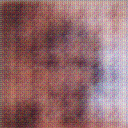
\includegraphics[width=150px]{500_fake_images/samples_5_45.png}%
\caption{A Close Up Of A Person Holding A Pair Of Scissors}%
\end{figure}

%
\end{document}